% Nallino, Part I p. 112: the figure of a solar eclipse, redrawn from the print: the circle ABCD of the
% half sum of the diameters and the disc of the Sun FKRL, both about E, the diameters CA and BD, the
% discs of the Moon at the beginning (centre S), the middle (centre G, a dot) and the end (centre Q),
% the lines EHQ, PQ, SM and ENS; the four quarters MERIDIES, SEPTENTRIONES, ORIENS (reading downward)
% and OCCIDENS (reading upward). Circles and lines are least-squares fits to the printed ink;
% coordinates are PDF points of master page 201 less the origin (120.24, 430.16), y downward.
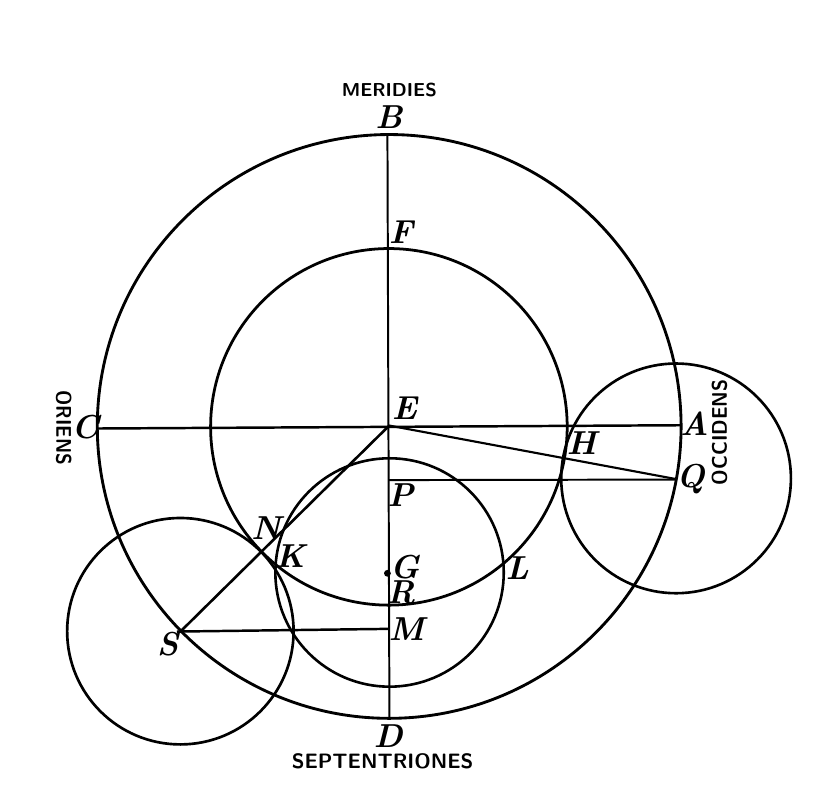
\begin{tikzpicture}[x=0.9851pt,y=-0.9851pt,line cap=butt,every node/.style={font=\fontsize{11.5}{11.5}\bfseries\itshape\selectfont,inner sep=0pt}]
\useasboundingbox (0,0) rectangle (285.00,275.00);
\draw[line width=1.03pt] (132.61,146.27) circle[radius=107.07];  % the circle ABCD of the half sum of the two diameters, centre E
\draw[line width=1.00pt] (132.50,146.42) circle[radius=65.40];  % the disc of the Sun FKRL, centre E
\draw[line width=0.94pt] (132.74,199.84) circle[radius=41.89];  % the disc of the Moon at the middle of the eclipse, centre G
\draw[line width=0.95pt] (237.84,165.32) circle[radius=42.13];  % the disc of the Moon at the end of the emersion, centre Q
\draw[line width=0.96pt] (56.01,221.38) circle[radius=41.53];  % the disc of the Moon at the beginning of the immersion, centre S
\draw[line width=0.89pt] (25.55,147.03) -- (239.67,145.83);  % the diameter CA (east to west)
\draw[line width=0.71pt] (131.96,39.20) -- (132.70,253.33);  % the diameter BD (south to north)
\draw[line width=0.77pt] (132.33,145.90) -- (237.74,165.56);  % the line EHQ
\draw[line width=0.71pt] (132.39,165.95) -- (237.63,165.76);  % the line PQ
\draw[line width=0.89pt] (54.76,221.51) -- (132.58,220.52);  % the line SM
\draw[line width=0.94pt] (132.33,146.23) -- (55.79,221.75);  % the line ENS
\draw[line width=0.10pt] (131.96,200.14) circle[radius=0.01];
\fill (131.96,200.14) circle[radius=1.25];
\node at (132.56,32.69) {B};
\node at (136.91,75.09) {F};
\node at (138.22,139.72) {E};
\node at (21.11,146.64) {C};
\node at (244.51,145.34) {A};
\node at (203.16,152.49) {H};
\node at (243.16,165.74) {Q};
\node at (136.76,171.44) {P};
\node at (87.46,183.74) {N};
\node at (96.29,193.80) {K};
\node at (138.31,197.79) {G};
\node at (136.94,207.04) {R};
\node at (179.61,198.14) {L};
\node at (51.31,226.02) {S};
\node at (138.93,220.75) {M};
\node at (132.21,259.94) {D};
\node at (132.67,22.93) {\normalfont\fontsize{8.5}{8.5}\sffamily\bfseries\selectfont \resizebox{34.31pt}{4.70pt}{MERIDIES}};
\node at (130.19,269.19) {\normalfont\fontsize{8.5}{8.5}\sffamily\bfseries\selectfont \resizebox{65.61pt}{5.22pt}{SEPTENTRIONES}};
\node[rotate=-90] at (13.25,146.81) {\normalfont\fontsize{8.5}{8.5}\sffamily\bfseries\selectfont \resizebox{26.86pt}{5.32pt}{ORIENS}};
\node[rotate=90] at (253.81,148.46) {\normalfont\fontsize{8.5}{8.5}\sffamily\bfseries\selectfont \resizebox{38.03pt}{5.32pt}{OCCIDENS}};
\end{tikzpicture}
